\documentclass[10pt,a4paper]{scrartcl}
\usepackage[utf8]{inputenc}
\usepackage{amsmath}
\usepackage{amsfonts}
\usepackage{amssymb}
\usepackage{graphicx}
\usepackage{geometry}
\usepackage{tabularx}
\usepackage[section]{placeins}
\geometry{a4paper, top=13mm, left=10mm, right=13mm, bottom=10mm, includefoot}
%\newcommand*{\myalign}[2]{\multicolumn{1}{#1}{#2}}
\newcolumntype{Y}{>{\centering\arraybackslash}X}
\begin{document}
	\title{The political economy of EU asylum policies}
	\subtitle{Results first time applications per capita}
	\author{Martina Burmann, Marcus Drometer and Romuald Méango}
	\maketitle


\tableofcontents

\clearpage
\FloatBarrier
\section{Summary Statistics}
\begin{table}[htbp]\centering \caption{Summary statistics\label{sumstat}}
\begin{tabular}{l c c c c c }\hline\hline
\multicolumn{1}{c}{Variable} & Obs & Mean & Std. Dev.
 & Min & Max  \\ \hline
Quarterly fist-time asylum applications & 23705 & 114.2 & 338.1 & 0 & 15330  \\
Quarterly first-time asylum applications per 10000 inhabitants & 23705 & .1 & .2 & 0 & 11.3  \\
(first) cabinet\_left\_right & 23705 & 5.6 & 1.5 & 2.8 & 8.2  \\
Political Terror Scale & 23705 & 3.3 & .9 & 1 & 5  \\
Civic Liberty (FHI) & 23705 & 4.6 & 1.4 & 2 & 7  \\
Political Rights (FHI) & 23705 & 4.9 & 1.7 & 1 & 7  \\
Quarterly civil war battle death (000s) & 23705 & .3 & 1.3 & 0 & 17.6  \\
Yearly real GDP per capita at origin & 23705 & 6440.8 & 5270.3 & 336.8 & 24039.1  \\
Distance from origin to destination & 23705 & 4395.2 & 2167.8 & 454 & 9680  \\
Migrant stock in 2000/1 & 23705 & 16452.5 & 74737.4 & 0 & 1272000  \\
Quarterly real GDP per capita at destination & 23705 & 8717.2 & 3203.3 & 1557.5 & 18025.9  \\
Quarterly unemployment rate at destination & 23705 & 7.8 & 3.9 & 2.4 & 26.9  \\
\hline\end{tabular}
\end{table}

 
\clearpage
\FloatBarrier
\section{Baseline Specification}
\begin{table}[!ht]\centering
\renewcommand{\arraystretch}{1.25}
\small
\def\sym#1{\ifmmode^{#1}\else\(^{#1}\)\fi}
\caption{Determinants of log(First time asylum applications per capita)}
\begin{tabular}{l*{3}{c}}
	\hline\hline
	\input{app_Table1.tex}
	\hline\hline
	\multicolumn{4}{l}{\footnotesize Standard errors in parentheses (\sym{*} \(p<0.05\), \sym{**} \(p<0.01\), \sym{***} \(p<0.001\))}\\
\end{tabular}
\end{table}

\clearpage
\textbf{Baseline Specification - Model 1}
\begin{figure}[!ht]
	\centering
	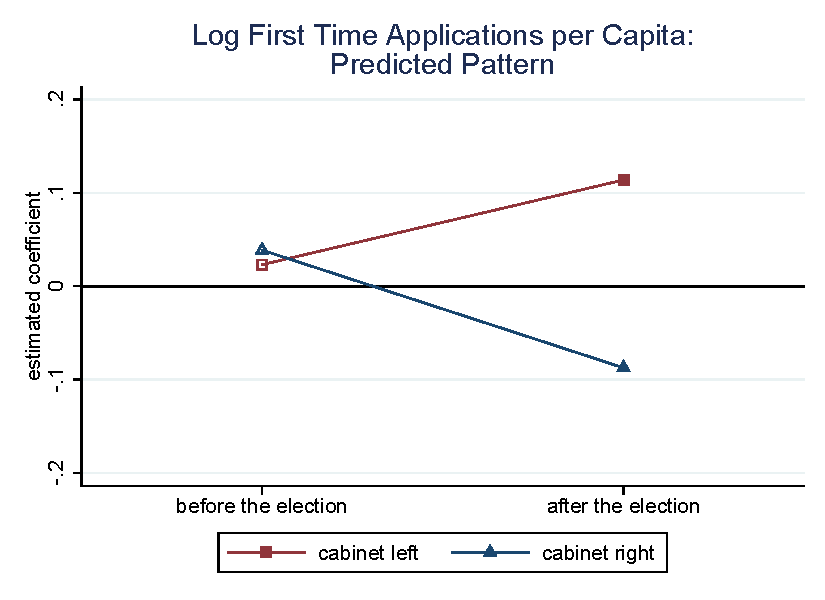
\includegraphics[width=1\textwidth]{app_Graph1.pdf}
	\caption{log First Time Asylum Applications per Capita: Predicted Pattern}
\end{figure}

\begin{table}[!ht]\centering
\renewcommand{\arraystretch}{1.25}
\def\sym#1{\ifmmode^{#1}\else\(^{#1}\)\fi}
\caption{Log First Time Applications per Capita: Predicted Pattern}
\begin{tabular}[]{l*{3}{c}}
\hline\hline
	\input{app_Graph1_Coeff.tex}
\hline\hline
\multicolumn{4}{c}{Standard errors in parentheses} \\
\multicolumn{4}{c}{\footnotesize (\sym{*} \(p<0.05\), \sym{**} \(p<0.01\), \sym{***} \(p<0.001\))}\\
\end{tabular}
\end{table}

\clearpage
\textbf{Baseline Specification - Model 2}
\begin{table}[!ht]\centering
	\scriptsize
	\renewcommand{\arraystretch}{1.1}
	\def\sym#1{\ifmmode^{#1}\else\(^{#1}\)\fi}
	\caption{Determinants of log(First time asylum applications per capita)}
	\begin{tabular}{l*{3}{c}}
		\hline\hline
		\input{app_Table2.tex}
		\hline\hline
		\multicolumn{4}{c}{\footnotesize Standard errors in parentheses (\sym{*} \(p<0.05\), \sym{**} \(p<0.01\), \sym{***} \(p<0.001\))}\\
	\end{tabular}
\end{table}



\clearpage
\textbf{Baseline Specification - Model 2}
\begin{figure}[!ht]
	\centering
	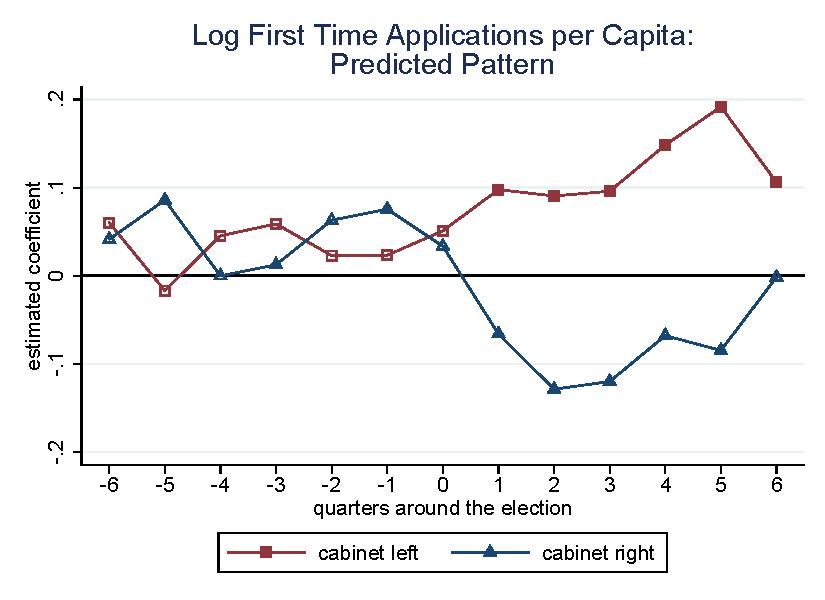
\includegraphics[width=0.7\textwidth]{app_Graph2.pdf}
	\caption{log First Time Asylum Applications per Capita: Predicted Pattern}
\end{figure}

\begin{table}[!ht]\centering
	\footnotesize
	\renewcommand{\arraystretch}{1.25}
	\def\sym#1{\ifmmode^{#1}\else\(^{#1}\)\fi}
	\caption{Log First Time Applications per Capita: Predicted Pattern}
	\begin{tabular}{l*{3}{c}}
		\hline\hline
		\input{app_Graph2_Coeff.tex}
		\hline\hline
		\multicolumn{4}{l}{\footnotesize Standard errors in parentheses (\sym{*} \(p<0.05\), \sym{**} \(p<0.01\), \sym{***} \(p<0.001\))}\\
	\end{tabular}
\end{table}


\FloatBarrier
\clearpage
\section{Robustness}
\subsection{Use destination, origin and time fixed effects}
\textbf{ R1: Use destination, origin and time fixed effects - Model 1}
\begin{figure}[!ht]
	\centering
	\includegraphics[width=1\textwidth]{app_Graph1R1.pdf}
	\caption{R1: log First Time Asylum Applications per Capita: Predicted Pattern}
\end{figure}

\begin{table}[!ht]\centering
	\renewcommand{\arraystretch}{1.25}
	\def\sym#1{\ifmmode^{#1}\else\(^{#1}\)\fi}
	\caption{R1: Log First Time Applications per Capita: Predicted Pattern}
	\begin{tabular}{l*{3}{c}}
		\hline\hline
		\input{app_Graph1R1_Coeff.tex}
		\hline\hline
		\multicolumn{4}{l}{\footnotesize Standard errors in parentheses (\sym{*} \(p<0.05\), \sym{**} \(p<0.01\), \sym{***} \(p<0.001\))}\\
	\end{tabular}
\end{table}

\clearpage
\textbf{ R1: Use destination, origin and time fixed effects - Model 2}
\begin{figure}[!ht]
	\centering
	\includegraphics[width=0.7\textwidth]{app_Graph2R1.pdf}
	\caption{R1: log First Time Asylum Applications per Capita: Predicted Pattern}
\end{figure}

\begin{table}[!ht]\centering
	\footnotesize
	\renewcommand{\arraystretch}{1.25}
	\def\sym#1{\ifmmode^{#1}\else\(^{#1}\)\fi}
	\caption{R1: Log First Time Applications per Capita: Predicted Pattern}
	\begin{tabular}{l*{3}{c}}
		\hline\hline
		\input{app_Graph2R1_Coeff.tex}
		\hline\hline
		\multicolumn{4}{l}{\footnotesize Standard errors in parentheses (\sym{*} \(p<0.05\), \sym{**} \(p<0.01\), \sym{***} \(p<0.001\))}\\
	\end{tabular}
\end{table}

\FloatBarrier
\clearpage
\subsection{Use destination and origin*time fixed effects}
\textbf{ R2: Use destination and origin*time fixed effects - Model 1}
\begin{figure}[!ht]
	\centering
	\includegraphics[width=1\textwidth]{app_Graph1R2.pdf}
	\caption{R2: log First Time Asylum Applications per Capita: Predicted Pattern}
\end{figure}

\begin{table}[!ht]\centering
	\renewcommand{\arraystretch}{1.25}
	\def\sym#1{\ifmmode^{#1}\else\(^{#1}\)\fi}
	\caption{R2: Log First Time Applications per Capita: Predicted Pattern}
	\begin{tabular}{l*{3}{c}}
		\hline\hline
		\input{app_Graph1R2_Coeff.tex}
		\hline\hline
		\multicolumn{4}{l}{\footnotesize Standard errors in parentheses} \\
		\multicolumn{4}{l}{\footnotesize(\sym{*} \(p<0.05\), \sym{**} \(p<0.01\), \sym{***} \(p<0.001\))}\\
	\end{tabular}
\end{table}

\clearpage
\textbf{ R2: Use destination and origin*time fixed effects - Model 2}
\begin{figure}[!ht]
	\centering
	\includegraphics[width=0.7\textwidth]{app_Graph2R2.pdf}
	\caption{R2: log First Time Asylum Applications per Capita: Predicted Pattern}
\end{figure}

\begin{table}[!ht]\centering
	\footnotesize
	\renewcommand{\arraystretch}{1.25}
	\def\sym#1{\ifmmode^{#1}\else\(^{#1}\)\fi}
	\caption{R2: Log First Time Applications per Capita: Predicted Pattern}
	\begin{tabular}{l*{3}{c}}
		\hline\hline
		\input{app_Graph2R2_Coeff.tex}
		\hline\hline
		\multicolumn{4}{l}{\footnotesize Standard errors in parentheses (\sym{*} \(p<0.05\), \sym{**} \(p<0.01\), \sym{***} \(p<0.001\))}\\
	\end{tabular}
\end{table}


\clearpage
\FloatBarrier
\subsection{Control for past applications}
\begin{table}[!ht]\centering
	\renewcommand{\arraystretch}{1.25}
	\small
	\def\sym#1{\ifmmode^{#1}\else\(^{#1}\)\fi}
	\caption{R3: Determinants of log(First time asylum applications per capita)}
	\begin{tabular}{l*{3}{c}}
		\hline\hline
		\input{app_Table1R3.tex}
		\hline\hline
		\multicolumn{4}{l}{\footnotesize Standard errors in parentheses (\sym{*} \(p<0.05\), \sym{**} \(p<0.01\), \sym{***} \(p<0.001\))}\\
	\end{tabular}
\end{table}

\clearpage
\textbf{R3: Control for past applications - Model 1}
\begin{figure}[!ht]
	\centering
	\includegraphics[width=1\textwidth]{app_Graph1R3.pdf}
	\caption{R3: log First Time Asylum Applications per Capita: Predicted Pattern}
\end{figure}

\begin{table}[!ht]\centering
	\renewcommand{\arraystretch}{1.25}
	\def\sym#1{\ifmmode^{#1}\else\(^{#1}\)\fi}
	\caption{R3: Log First Time Applications per Capita: Predicted Pattern}
	\begin{tabular}{l*{3}{c}}
		\hline\hline
		\input{app_Graph1R3_Coeff.tex}
		\hline\hline
		\multicolumn{4}{l}{\footnotesize Standard errors in parentheses (\sym{*} \(p<0.05\), \sym{**} \(p<0.01\), \sym{***} \(p<0.001\))}\\
	\end{tabular}
\end{table}

\clearpage
\textbf{R3: Control for past applications - Model 2}
\begin{figure}[!ht]
	\centering
	\includegraphics[width=0.7\textwidth]{app_Graph2R3.pdf}
	\caption{R3: log First Time Asylum Applications per Capita: Predicted Pattern}
\end{figure}

\begin{table}[!ht]\centering
	\footnotesize
	\renewcommand{\arraystretch}{1.25}
	\def\sym#1{\ifmmode^{#1}\else\(^{#1}\)\fi}
	\caption{R3: Log First Time Applications per Capita: Predicted Pattern}
	\begin{tabular}{l*{3}{c}}
		\hline\hline
		\input{app_Graph2R3_Coeff.tex}
		\hline\hline
		\multicolumn{4}{l}{\footnotesize Standard errors in parentheses (\sym{*} \(p<0.05\), \sym{**} \(p<0.01\), \sym{***} \(p<0.001\))}\\
	\end{tabular}
\end{table}

\clearpage
\FloatBarrier
\subsection{Control for cabinet position}
\begin{table}[!ht]\centering
	\renewcommand{\arraystretch}{1.25}
	\small
	\def\sym#1{\ifmmode^{#1}\else\(^{#1}\)\fi}
	\caption{R4: Determinants of log(First time asylum applications per capita)}
	\begin{tabular}{l*{3}{c}}
		\hline\hline
		\input{app_Table1R4.tex}
		\hline\hline
		\multicolumn{4}{l}{\footnotesize Standard errors in parentheses (\sym{*} \(p<0.05\), \sym{**} \(p<0.01\), \sym{***} \(p<0.001\))}\\
	\end{tabular}
\end{table}

\clearpage
\textbf{R4: Control for cabinet position - Model 1}
\begin{figure}[!ht]
	\centering
	\includegraphics[width=1\textwidth]{app_Graph1R4.pdf}
	\caption{R4: log First Time Asylum Applications per Capita: Predicted Pattern}
\end{figure}

\begin{table}[!ht]\centering
	\renewcommand{\arraystretch}{1.25}
	\def\sym#1{\ifmmode^{#1}\else\(^{#1}\)\fi}
	\caption{R4: Log First Time Applications per Capita: Predicted Pattern}
	\begin{tabular}{l*{3}{c}}
		\hline\hline
		\input{app_Graph1R4_Coeff.tex}
		\hline\hline
		\multicolumn{4}{l}{\footnotesize Standard errors in parentheses (\sym{*} \(p<0.05\), \sym{**} \(p<0.01\), \sym{***} \(p<0.001\))}\\
	\end{tabular}
\end{table}

\clearpage
\textbf{R4: Control for cabinet position - Model 2}
\begin{figure}[!ht]
	\centering
	\includegraphics[width=0.7\textwidth]{app_Graph2R4.pdf}
	\caption{R4: log First Time Asylum Applications per Capita: Predicted Pattern}
\end{figure}

\begin{table}[!ht]\centering
	\footnotesize
	\renewcommand{\arraystretch}{1.25}
	\def\sym#1{\ifmmode^{#1}\else\(^{#1}\)\fi}
	\caption{R4: Log First Time Applications per Capita: Predicted Pattern}
	\begin{tabular}{l*{3}{c}}
		\hline\hline
		\input{app_Graph2R4_Coeff.tex}
		\hline\hline
		\multicolumn{4}{l}{\footnotesize Standard errors in parentheses (\sym{*} \(p<0.05\), \sym{**} \(p<0.01\), \sym{***} \(p<0.001\))}\\
	\end{tabular}
\end{table}


\clearpage
\FloatBarrier
\subsection{Use log first time applications per capita in origin country as dependent variable}
\begin{table}[!ht]\centering
	\renewcommand{\arraystretch}{1.25}
	\small
	\def\sym#1{\ifmmode^{#1}\else\(^{#1}\)\fi}
	\caption{R5: Determinants of log(First time asylum applications per capita)}
	\begin{tabular}{l*{3}{c}}
		\hline\hline
		\input{app_Table1R5.tex}
		\hline\hline
		\multicolumn{4}{l}{\footnotesize Standard errors in parentheses (\sym{*} \(p<0.05\), \sym{**} \(p<0.01\), \sym{***} \(p<0.001\))}\\
	\end{tabular}
\end{table}

\clearpage
\textbf{R5: Use log first time applications per capita in origin country as dependent variable - Model 1}
\begin{figure}[!ht]
	\centering
	\includegraphics[width=1\textwidth]{app_Graph1R5.pdf}
	\caption{R5: log First Time Asylum Applications per Capita: Predicted Pattern}
\end{figure}

\begin{table}[!ht]\centering
	\renewcommand{\arraystretch}{1.25}
	\def\sym#1{\ifmmode^{#1}\else\(^{#1}\)\fi}
	\caption{R5: Log First Time Applications per Capita: Predicted Pattern}
	\begin{tabular}{l*{3}{c}}
		\hline\hline
		\input{app_Graph1R5_Coeff.tex}
		\hline\hline
		\multicolumn{4}{l}{\footnotesize Standard errors in parentheses (\sym{*} \(p<0.05\), \sym{**} \(p<0.01\), \sym{***} \(p<0.001\))}\\
	\end{tabular}
\end{table}

\clearpage
\textbf{R5: Use log first time applications per capita in origin country as dependent variable - Model 2}
\begin{figure}[!ht]
	\centering
	\includegraphics[width=0.7\textwidth]{app_Graph2R5.pdf}
	\caption{R5: log First Time Asylum Applications per Capita: Predicted Pattern}
\end{figure}

\begin{table}[!ht]\centering
	\footnotesize
	\renewcommand{\arraystretch}{1.25}
	\def\sym#1{\ifmmode^{#1}\else\(^{#1}\)\fi}
	\caption{R5: Log First Time Applications per Capita: Predicted Pattern}
	\begin{tabular}{l*{3}{c}}
		\hline\hline
		\input{app_Graph2R5_Coeff.tex}
		\hline\hline
		\multicolumn{4}{l}{\footnotesize Standard errors in parentheses (\sym{*} \(p<0.05\), \sym{**} \(p<0.01\), \sym{***} \(p<0.001\))}\\
	\end{tabular}
\end{table}



\clearpage
\FloatBarrier
\subsection{Don't use lagged origin country variables}
\begin{table}[!ht]\centering
	\renewcommand{\arraystretch}{1.25}
	\small
	\def\sym#1{\ifmmode^{#1}\else\(^{#1}\)\fi}
	\caption{R6: Determinants of log(First time asylum applications per capita)}
	\begin{tabular}{l*{3}{c}}
		\hline\hline
		\input{app_Table1R6.tex}
		\hline\hline
		\multicolumn{4}{l}{\footnotesize Standard errors in parentheses (\sym{*} \(p<0.05\), \sym{**} \(p<0.01\), \sym{***} \(p<0.001\))}\\
	\end{tabular}
\end{table}

\clearpage
\textbf{R6: Don't use lagged origin country variables - Model 1}
\begin{figure}[!ht]
	\centering
	\includegraphics[width=1\textwidth]{app_Graph1R6.pdf}
	\caption{R6: log First Time Asylum Applications per Capita: Predicted Pattern}
\end{figure}

\begin{table}[!ht]\centering
	\renewcommand{\arraystretch}{1.25}
	\def\sym#1{\ifmmode^{#1}\else\(^{#1}\)\fi}
	\caption{R6: Log First Time Applications per Capita: Predicted Pattern}
	\begin{tabular}{l*{3}{c}}
		\hline\hline
		\input{app_Graph1R6_Coeff.tex}
		\hline\hline
		\multicolumn{4}{l}{\footnotesize Standard errors in parentheses (\sym{*} \(p<0.05\), \sym{**} \(p<0.01\), \sym{***} \(p<0.001\))}\\
	\end{tabular}
\end{table}

\clearpage
\textbf{R6: Don't use lagged origin country variables - Model 2}
\begin{figure}[!ht]
	\centering
	\includegraphics[width=0.7\textwidth]{app_Graph2R6.pdf}
	\caption{R6: log First Time Asylum Applications per Capita: Predicted Pattern}
\end{figure}

\begin{table}[!ht]\centering
	\footnotesize
	\renewcommand{\arraystretch}{1.25}
	\def\sym#1{\ifmmode^{#1}\else\(^{#1}\)\fi}
	\caption{R6: Log First Time Applications per Capita: Predicted Pattern}
	\begin{tabular}{l*{3}{c}}
		\hline\hline
		\input{app_Graph2R6_Coeff.tex}
		\hline\hline
		\multicolumn{4}{l}{\footnotesize Standard errors in parentheses (\sym{*} \(p<0.05\), \sym{**} \(p<0.01\), \sym{***} \(p<0.001\))}\\
	\end{tabular}
\end{table}

\clearpage
\subsection{Include a post 2007 dummy}
\begin{table}[!ht]\centering
	\renewcommand{\arraystretch}{1.25}
	\small
	\def\sym#1{\ifmmode^{#1}\else\(^{#1}\)\fi}
	\caption{R7: Determinants of log(First time asylum applications per capita)}
	\begin{tabular}{l*{3}{c}}
		\hline\hline
		\input{app_Table1R7.tex}
		\hline\hline
		\multicolumn{4}{l}{\footnotesize Standard errors in parentheses (\sym{*} \(p<0.05\), \sym{**} \(p<0.01\), \sym{***} \(p<0.001\))}\\
	\end{tabular}
\end{table}

\clearpage
\textbf{R7: Include a post 2007 dummy - Model 1}
\begin{figure}[!ht]
	\centering
	\includegraphics[width=1\textwidth]{app_Graph1R7.pdf}
	\caption{R7: log First Time Asylum Applications per Capita: Predicted Pattern}
\end{figure}

\begin{table}[!ht]\centering
	\renewcommand{\arraystretch}{1.25}
	\def\sym#1{\ifmmode^{#1}\else\(^{#1}\)\fi}
	\caption{R7: Log First Time Applications per Capita: Predicted Pattern}
	\begin{tabular}{l*{3}{c}}
		\hline\hline
		\input{app_Graph1R7_Coeff.tex}
		\hline\hline
		\multicolumn{4}{l}{\footnotesize Standard errors in parentheses (\sym{*} \(p<0.05\), \sym{**} \(p<0.01\), \sym{***} \(p<0.001\))}\\
	\end{tabular}
\end{table}

\clearpage
\textbf{R7: Include a post 2007 dummy - Model 2}
\begin{figure}[!ht]
	\centering
	\includegraphics[width=0.7\textwidth]{app_Graph2R7.pdf}
	\caption{R7: log First Time Asylum Applications per Capita: Predicted Pattern}
\end{figure}

\begin{table}[!ht]\centering
	\footnotesize
	\renewcommand{\arraystretch}{1.25}
	\def\sym#1{\ifmmode^{#1}\else\(^{#1}\)\fi}
	\caption{R7: Log First Time Applications per Capita: Predicted Pattern}
	\begin{tabular}{l*{3}{c}}
		\hline\hline
		\input{app_Graph2R7_Coeff.tex}
		\hline\hline
		\multicolumn{4}{l}{\footnotesize Standard errors in parentheses (\sym{*} \(p<0.05\), \sym{**} \(p<0.01\), \sym{***} \(p<0.001\))}\\
	\end{tabular}
\end{table}


\clearpage
\subsection{Cluster standard errors on destionation*origin level}
\begin{table}[!ht]\centering
	\renewcommand{\arraystretch}{1.25}
	\small
	\def\sym#1{\ifmmode^{#1}\else\(^{#1}\)\fi}
	\caption{R8: Determinants of log(First time asylum applications per capita)}
	\begin{tabular}{l*{3}{c}}
		\hline\hline
		\input{app_Table1R8.tex}
		\hline\hline
		\multicolumn{4}{l}{\footnotesize Standard errors in parentheses (\sym{*} \(p<0.05\), \sym{**} \(p<0.01\), \sym{***} \(p<0.001\))}\\
	\end{tabular}
\end{table}

\clearpage
\textbf{R8: Cluster standard errors on destionation*origin level - Model 1}
\begin{figure}[!ht]
	\centering
	\includegraphics[width=1\textwidth]{app_Graph1R8.pdf}
	\caption{R8: log First Time Asylum Applications per Capita: Predicted Pattern}
\end{figure}

\begin{table}[!ht]\centering
	\renewcommand{\arraystretch}{1.25}
	\def\sym#1{\ifmmode^{#1}\else\(^{#1}\)\fi}
	\caption{R8: Log First Time Applications per Capita: Predicted Pattern}
	\begin{tabular}{l*{3}{c}}
		\hline\hline
		\input{app_Graph1R8_Coeff.tex}
		\hline\hline
		\multicolumn{4}{l}{\footnotesize Standard errors in parentheses (\sym{*} \(p<0.05\), \sym{**} \(p<0.01\), \sym{***} \(p<0.001\))}\\
	\end{tabular}
\end{table}

\clearpage
\textbf{R8: Cluster standard errors on destionation*origin level - Model 2}
\begin{figure}[!ht]
	\centering
	\includegraphics[width=0.7\textwidth]{app_Graph2R8.pdf}
	\caption{R8: log First Time Asylum Applications per Capita: Predicted Pattern}
\end{figure}

\begin{table}[!ht]\centering
	\footnotesize
	\renewcommand{\arraystretch}{1.25}
	\def\sym#1{\ifmmode^{#1}\else\(^{#1}\)\fi}
	\caption{R8: Log First Time Applications per Capita: Predicted Pattern}
	\begin{tabular}{l*{3}{c}}
		\hline\hline
		\input{app_Graph2R8_Coeff.tex}
		\hline\hline
		\multicolumn{4}{l}{\footnotesize Standard errors in parentheses (\sym{*} \(p<0.05\), \sym{**} \(p<0.01\), \sym{***} \(p<0.001\))}\\
	\end{tabular}
\end{table}

\clearpage
\FloatBarrier
\subsection{Use normalized cabinet position to determine cabinet left-right dummies}
\begin{table}[!ht]\centering
	\renewcommand{\arraystretch}{1.25}
	\small
	\def\sym#1{\ifmmode^{#1}\else\(^{#1}\)\fi}
	\caption{R9: Determinants of log(First time asylum applications per capita)}
	\begin{tabular}{l*{3}{c}}
		\hline\hline
		\input{app_Table1R9.tex}
		\hline\hline
		\multicolumn{4}{l}{\footnotesize Standard errors in parentheses (\sym{*} \(p<0.05\), \sym{**} \(p<0.01\), \sym{***} \(p<0.001\))}\\
	\end{tabular}
\end{table}

\clearpage
\textbf{R9: Use normalized cabinet position to determine cabinet left-right dummies - Model 1}
\begin{figure}[!ht]
	\centering
	\includegraphics[width=1\textwidth]{app_Graph1R9.pdf}
	\caption{R9: log First Time Asylum Applications per Capita: Predicted Pattern}
\end{figure}

\begin{table}[!ht]\centering
	\renewcommand{\arraystretch}{1.25}
	\def\sym#1{\ifmmode^{#1}\else\(^{#1}\)\fi}
	\caption{R9: Log First Time Applications per Capita: Predicted Pattern}
	\begin{tabular}{l*{3}{c}}
		\hline\hline
		\input{app_Graph1R9_Coeff.tex}
		\hline\hline
		\multicolumn{4}{l}{\footnotesize Standard errors in parentheses (\sym{*} \(p<0.05\), \sym{**} \(p<0.01\), \sym{***} \(p<0.001\))}\\
	\end{tabular}
\end{table}

\clearpage
\textbf{R9: Use normalized cabinet position to determine cabinet left-right dummies - Model 2}
\begin{figure}[!ht]
	\centering
	\includegraphics[width=0.7\textwidth]{app_Graph2R9.pdf}
	\caption{R9: log First Time Asylum Applications per Capita: Predicted Pattern}
\end{figure}

\begin{table}[!ht]\centering
	\footnotesize
	\renewcommand{\arraystretch}{1.25}
	\def\sym#1{\ifmmode^{#1}\else\(^{#1}\)\fi}
	\caption{R9: Log First Time Applications per Capita: Predicted Pattern}
	\begin{tabular}{l*{3}{c}}
		\hline\hline
		\input{app_Graph2R9_Coeff.tex}
		\hline\hline
		\multicolumn{4}{l}{\footnotesize Standard errors in parentheses (\sym{*} \(p<0.05\), \sym{**} \(p<0.01\), \sym{***} \(p<0.001\))}\\
	\end{tabular}
\end{table}


\clearpage
\subsection{Do not impute first time application data for 2008 and 2009}
\begin{table}[!ht]\centering
	\renewcommand{\arraystretch}{1.25}
	\small
	\def\sym#1{\ifmmode^{#1}\else\(^{#1}\)\fi}
	\caption{R10: Determinants of log(First time asylum applications per capita)}
	\begin{tabular}{l*{3}{c}}
		\hline\hline
		\input{app_Table1R10.tex}
		\hline\hline
		\multicolumn{4}{l}{\footnotesize Standard errors in parentheses (\sym{*} \(p<0.05\), \sym{**} \(p<0.01\), \sym{***} \(p<0.001\))}\\
	\end{tabular}
\end{table}

\clearpage
\textbf{R10: Do not impute first time application data for 2008 and 2009 - Model 1}
\begin{figure}[!ht]
	\centering
	\includegraphics[width=1\textwidth]{app_Graph1R10.pdf}
	\caption{R10: log First Time Asylum Applications per Capita: Predicted Pattern}
\end{figure}

\begin{table}[!ht]\centering
	\renewcommand{\arraystretch}{1.25}
	\def\sym#1{\ifmmode^{#1}\else\(^{#1}\)\fi}
	\caption{R10: Log First Time Applications per Capita: Predicted Pattern}
	\begin{tabular}{l*{3}{c}}
		\hline\hline
		\input{app_Graph1R10_Coeff.tex}
		\hline\hline
		\multicolumn{4}{l}{\footnotesize Standard errors in parentheses (\sym{*} \(p<0.05\), \sym{**} \(p<0.01\), \sym{***} \(p<0.001\))}\\
	\end{tabular}
\end{table}

\clearpage
\textbf{R10: Do not impute first time application data for 2008 and 2009 - Model 2}
\begin{figure}[!ht]
	\centering
	\includegraphics[width=0.7\textwidth]{app_Graph2R10.pdf}
	\caption{R10: log First Time Asylum Applications per Capita: Predicted Pattern}
\end{figure}

\begin{table}[!ht]\centering
	\footnotesize
	\renewcommand{\arraystretch}{1.25}
	\def\sym#1{\ifmmode^{#1}\else\(^{#1}\)\fi}
	\caption{R10: Log First Time Applications per Capita: Predicted Pattern}
	\begin{tabular}{l*{3}{c}}
		\hline\hline
		\input{app_Graph2R10_Coeff.tex}
		\hline\hline
		\multicolumn{4}{l}{\footnotesize Standard errors in parentheses (\sym{*} \(p<0.05\), \sym{**} \(p<0.01\), \sym{***} \(p<0.001\))}\\
	\end{tabular}
\end{table}

\clearpage
\FloatBarrier
\subsection{Drop country pairs with less than 1 first time application per quarter on average}
\begin{table}[!ht]\centering
	\renewcommand{\arraystretch}{1.25}
	\small
	\def\sym#1{\ifmmode^{#1}\else\(^{#1}\)\fi}
	\caption{R11: Determinants of log(First time asylum applications per capita)}
	\begin{tabular}{l*{3}{c}}
		\hline\hline
		\input{app_Table1R11.tex}
		\hline\hline
		\multicolumn{4}{l}{\footnotesize Standard errors in parentheses (\sym{*} \(p<0.05\), \sym{**} \(p<0.01\), \sym{***} \(p<0.001\))}\\
	\end{tabular}
\end{table}

\clearpage
\textbf{R11: Drop country pairs with less than 1 first time application per quarter on average - Model 1}
\begin{figure}[!ht]
	\centering
	\includegraphics[width=1\textwidth]{app_Graph1R11.pdf}
	\caption{R11: log First Time Asylum Applications per Capita: Predicted Pattern}
\end{figure}

\begin{table}[!ht]\centering
	\renewcommand{\arraystretch}{1.25}
	\def\sym#1{\ifmmode^{#1}\else\(^{#1}\)\fi}
	\caption{R11: Log First Time Applications per Capita: Predicted Pattern}
	\begin{tabular}{l*{3}{c}}
		\hline\hline
		\input{app_Graph1R11_Coeff.tex}
		\hline\hline
		\multicolumn{4}{l}{\footnotesize Standard errors in parentheses (\sym{*} \(p<0.05\), \sym{**} \(p<0.01\), \sym{***} \(p<0.001\))}\\
	\end{tabular}
\end{table}

\clearpage
\textbf{R11: Drop country pairs with less than 1 first time application per quarter on average - Model 2}
\begin{figure}[!ht]
	\centering
	\includegraphics[width=0.7\textwidth]{app_Graph2R11.pdf}
	\caption{R11: log First Time Asylum Applications per Capita: Predicted Pattern}
\end{figure}

\begin{table}[!ht]\centering
	\footnotesize
	\renewcommand{\arraystretch}{1.25}
	\def\sym#1{\ifmmode^{#1}\else\(^{#1}\)\fi}
	\caption{R11: Log First Time Applications per Capita: Predicted Pattern}
	\begin{tabular}{l*{3}{c}}
		\hline\hline
		\input{app_Graph2R11_Coeff.tex}
		\hline\hline
		\multicolumn{4}{l}{\footnotesize Standard errors in parentheses (\sym{*} \(p<0.05\), \sym{**} \(p<0.01\), \sym{***} \(p<0.001\))}\\
	\end{tabular}
\end{table}

\clearpage
\subsection{Drop country pairs with less than 3 first time applications per quarter on average}
\begin{table}[!ht]\centering
	\renewcommand{\arraystretch}{1.25}
	\small
	\def\sym#1{\ifmmode^{#1}\else\(^{#1}\)\fi}
	\caption{R12: Determinants of log(First time asylum applications per capita)}
	\begin{tabular}{l*{3}{c}}
		\hline\hline
		\input{app_Table1R12.tex}
		\hline\hline
		\multicolumn{4}{l}{\footnotesize Standard errors in parentheses (\sym{*} \(p<0.05\), \sym{**} \(p<0.01\), \sym{***} \(p<0.001\))}\\
	\end{tabular}
\end{table}

\clearpage
\textbf{R12: Drop country pairs with less than 3 first time applications per quarter on average - Model 1}
\begin{figure}[!ht]
	\centering
	\includegraphics[width=1\textwidth]{app_Graph1R12.pdf}
	\caption{R12: log First Time Asylum Applications per Capita: Predicted Pattern}
\end{figure}

\begin{table}[!ht]\centering
	\renewcommand{\arraystretch}{1.25}
	\def\sym#1{\ifmmode^{#1}\else\(^{#1}\)\fi}
	\caption{R12: Log First Time Applications per Capita: Predicted Pattern}
	\begin{tabular}{l*{3}{c}}
		\hline\hline
		\input{app_Graph1R12_Coeff.tex}
		\hline\hline
		\multicolumn{4}{l}{\footnotesize Standard errors in parentheses (\sym{*} \(p<0.05\), \sym{**} \(p<0.01\), \sym{***} \(p<0.001\))}\\
	\end{tabular}
\end{table}

\clearpage
\textbf{R12: Drop country pairs with less than 3 first time applications per quarter on average - Model 2}
\begin{figure}[!ht]
	\centering
	\includegraphics[width=0.7\textwidth]{app_Graph2R12.pdf}
	\caption{R12: log First Time Asylum Applications per Capita: Predicted Pattern}
\end{figure}

\begin{table}[!ht]\centering
	\footnotesize
	\renewcommand{\arraystretch}{1.25}
	\def\sym#1{\ifmmode^{#1}\else\(^{#1}\)\fi}
	\caption{R12: Log First Time Applications per Capita: Predicted Pattern}
	\begin{tabular}{l*{3}{c}}
		\hline\hline
		\input{app_Graph2R12_Coeff.tex}
		\hline\hline
		\multicolumn{4}{l}{\footnotesize Standard errors in parentheses (\sym{*} \(p<0.05\), \sym{**} \(p<0.01\), \sym{***} \(p<0.001\))}\\
	\end{tabular}
\end{table}

\clearpage
\subsection{Use only 5 quarters around the election}
\begin{table}[!ht]\centering
	\renewcommand{\arraystretch}{1.25}
	\small
	\def\sym#1{\ifmmode^{#1}\else\(^{#1}\)\fi}
	\caption{R13: Determinants of log(First time asylum applications per capita)}
	\begin{tabular}{l*{3}{c}}
		\hline\hline
		\input{app_Table1R13.tex}
		\hline\hline
		\multicolumn{4}{l}{\footnotesize Standard errors in parentheses (\sym{*} \(p<0.05\), \sym{**} \(p<0.01\), \sym{***} \(p<0.001\))}\\
	\end{tabular}
\end{table}

\clearpage
\textbf{R13: Use only 5 quarters around the election - Model 1}
\begin{figure}[!ht]
	\centering
	\includegraphics[width=1\textwidth]{app_Graph1R13.pdf}
	\caption{R13: log First Time Asylum Applications per Capita: Predicted Pattern}
\end{figure}

\begin{table}[!ht]\centering
	\renewcommand{\arraystretch}{1.25}
	\def\sym#1{\ifmmode^{#1}\else\(^{#1}\)\fi}
	\caption{R13: Log First Time Applications per Capita: Predicted Pattern}
	\begin{tabular}{l*{3}{c}}
		\hline\hline
		\input{app_Graph1R13_Coeff.tex}
		\hline\hline
		\multicolumn{4}{l}{\footnotesize Standard errors in parentheses (\sym{*} \(p<0.05\), \sym{**} \(p<0.01\), \sym{***} \(p<0.001\))}\\
	\end{tabular}
\end{table}

\clearpage
\textbf{R13: Use only 5 quarters around the election - Model 2}
\begin{figure}[!ht]
	\centering
	\includegraphics[width=0.7\textwidth]{app_Graph2R13.pdf}
	\caption{R13: log First Time Asylum Applications per Capita: Predicted Pattern}
\end{figure}

\begin{table}[!ht]\centering
	\footnotesize
	\renewcommand{\arraystretch}{1.25}
	\def\sym#1{\ifmmode^{#1}\else\(^{#1}\)\fi}
	\caption{R13: Log First Time Applications per Capita: Predicted Pattern}
	\begin{tabular}{l*{3}{c}}
		\hline\hline
		\input{app_Graph2R13_Coeff.tex}
		\hline\hline
		\multicolumn{4}{l}{\footnotesize Standard errors in parentheses (\sym{*} \(p<0.05\), \sym{**} \(p<0.01\), \sym{***} \(p<0.001\))}\\
	\end{tabular}
\end{table}

\clearpage
\subsection{Use only 4 quarters around the election}
\begin{table}[!ht]\centering
	\renewcommand{\arraystretch}{1.25}
	\small
	\def\sym#1{\ifmmode^{#1}\else\(^{#1}\)\fi}
	\caption{R14: Determinants of log(First time asylum applications per capita)}
	\begin{tabular}{l*{3}{c}}
		\hline\hline
		\input{app_Table1R14.tex}
		\hline\hline
		\multicolumn{4}{l}{\footnotesize Standard errors in parentheses (\sym{*} \(p<0.05\), \sym{**} \(p<0.01\), \sym{***} \(p<0.001\))}\\
	\end{tabular}
\end{table}

\clearpage
\textbf{R14: Use only 4 quarters around the election - Model 1}
\begin{figure}[!ht]
	\centering
	\includegraphics[width=1\textwidth]{app_Graph1R14.pdf}
	\caption{R14: log First Time Asylum Applications per Capita: Predicted Pattern}
\end{figure}

\begin{table}[!ht]\centering
	\renewcommand{\arraystretch}{1.25}
	\def\sym#1{\ifmmode^{#1}\else\(^{#1}\)\fi}
	\caption{R14: Log First Time Applications per Capita: Predicted Pattern}
	\begin{tabular}{l*{3}{c}}
		\hline\hline
		\input{app_Graph1R14_Coeff.tex}
		\hline\hline
		\multicolumn{4}{l}{\footnotesize Standard errors in parentheses (\sym{*} \(p<0.05\), \sym{**} \(p<0.01\), \sym{***} \(p<0.001\))}\\
	\end{tabular}
\end{table}

\clearpage
\textbf{R14: Use only 4 quarters around the election - Model 2}
\begin{figure}[!ht]
	\centering
	\includegraphics[width=0.7\textwidth]{app_Graph2R14.pdf}
	\caption{R14: log First Time Asylum Applications per Capita: Predicted Pattern}
\end{figure}

\begin{table}[!ht]\centering
	\footnotesize
	\renewcommand{\arraystretch}{1.25}
	\def\sym#1{\ifmmode^{#1}\else\(^{#1}\)\fi}
	\caption{R14: Log First Time Applications per Capita: Predicted Pattern}
	\begin{tabular}{l*{3}{c}}
		\hline\hline
		\input{app_Graph2R14_Coeff.tex}
		\hline\hline
		\multicolumn{4}{l}{\footnotesize Standard errors in parentheses (\sym{*} \(p<0.05\), \sym{**} \(p<0.01\), \sym{***} \(p<0.001\))}\\
	\end{tabular}
\end{table}


\clearpage
\subsection{Use data for all years 2002-2016}
\begin{table}[!ht]\centering
	\renewcommand{\arraystretch}{1.25}
	\small
	\def\sym#1{\ifmmode^{#1}\else\(^{#1}\)\fi}
	\caption{R15: Determinants of log(First time asylum applications per capita)}
	\begin{tabular}{l*{3}{c}}
		\hline\hline
		\input{app_Table1R15.tex}
		\hline\hline
		\multicolumn{4}{l}{\footnotesize Standard errors in parentheses (\sym{*} \(p<0.05\), \sym{**} \(p<0.01\), \sym{***} \(p<0.001\))}\\
	\end{tabular}
\end{table}

\clearpage
\textbf{R15: Use data for all years 2002-2016 - Model 1}
\begin{figure}[!ht]
	\centering
	\includegraphics[width=1\textwidth]{app_Graph1R15.pdf}
	\caption{R15: log First Time Asylum Applications per Capita: Predicted Pattern}
\end{figure}

\begin{table}[!ht]\centering
	\renewcommand{\arraystretch}{1.25}
	\def\sym#1{\ifmmode^{#1}\else\(^{#1}\)\fi}
	\caption{R15: Log First Time Applications per Capita: Predicted Pattern}
	\begin{tabular}{l*{3}{c}}
		\hline\hline
		\input{app_Graph1R15_Coeff.tex}
		\hline\hline
		\multicolumn{4}{l}{\footnotesize Standard errors in parentheses (\sym{*} \(p<0.05\), \sym{**} \(p<0.01\), \sym{***} \(p<0.001\))}\\
	\end{tabular}
\end{table}

\clearpage
\textbf{R15: Use data for all years 2002-2016 - Model 2}
\begin{figure}[!ht]
	\centering
	\includegraphics[width=0.7\textwidth]{app_Graph2R15.pdf}
	\caption{R15: log First Time Asylum Applications per Capita: Predicted Pattern}
\end{figure}

\begin{table}[!ht]\centering
	\footnotesize
	\renewcommand{\arraystretch}{1.25}
	\def\sym#1{\ifmmode^{#1}\else\(^{#1}\)\fi}
	\caption{R15: Log First Time Applications per Capita: Predicted Pattern}
	\begin{tabular}{l*{3}{c}}
		\hline\hline
		\input{app_Graph2R15_Coeff.tex}
		\hline\hline
		\multicolumn{4}{l}{\footnotesize Standard errors in parentheses (\sym{*} \(p<0.05\), \sym{**} \(p<0.01\), \sym{***} \(p<0.001\))}\\
	\end{tabular}
\end{table}


\clearpage
\subsection{Use all countries with less than two years missing data}
add Estonia, Latvia, Portugal, Slovenia, Cyprus, Lithuania, Malta
\begin{table}[!ht]\centering
	\renewcommand{\arraystretch}{1.25}
	\small
	\def\sym#1{\ifmmode^{#1}\else\(^{#1}\)\fi}
	\caption{R16: Determinants of log(First time asylum applications per capita)}
	\begin{tabular}{l*{3}{c}}
		\hline\hline
		\input{app_Table1R16.tex}
		\hline\hline
		\multicolumn{4}{l}{\footnotesize Standard errors in parentheses (\sym{*} \(p<0.05\), \sym{**} \(p<0.01\), \sym{***} \(p<0.001\))}\\
	\end{tabular}
\end{table}

\clearpage
\textbf{R16: Use all countries with less than two years missing data - Model 1}
\begin{figure}[!ht]
	\centering
	\includegraphics[width=1\textwidth]{app_Graph1R16.pdf}
	\caption{R16: log First Time Asylum Applications per Capita: Predicted Pattern}
\end{figure}

\begin{table}[!ht]\centering
	\renewcommand{\arraystretch}{1.25}
	\def\sym#1{\ifmmode^{#1}\else\(^{#1}\)\fi}
	\caption{R16: Log First Time Applications per Capita: Predicted Pattern}
	\begin{tabular}{l*{3}{c}}
		\hline\hline
		\input{app_Graph1R16_Coeff.tex}
		\hline\hline
		\multicolumn{4}{l}{\footnotesize Standard errors in parentheses (\sym{*} \(p<0.05\), \sym{**} \(p<0.01\), \sym{***} \(p<0.001\))}\\
	\end{tabular}
\end{table}

\clearpage
\textbf{R16: Use all countries with less than two years missing data - Model 2}
\begin{figure}[!ht]
	\centering
	\includegraphics[width=0.7\textwidth]{app_Graph2R16.pdf}
	\caption{R16: log First Time Asylum Applications per Capita: Predicted Pattern}
\end{figure}

\begin{table}[!ht]\centering
	\footnotesize
	\renewcommand{\arraystretch}{1.25}
	\def\sym#1{\ifmmode^{#1}\else\(^{#1}\)\fi}
	\caption{R16: Log First Time Applications per Capita: Predicted Pattern}
	\begin{tabular}{l*{3}{c}}
		\hline\hline
		\input{app_Graph2R16_Coeff.tex}
		\hline\hline
		\multicolumn{4}{l}{\footnotesize Standard errors in parentheses (\sym{*} \(p<0.05\), \sym{**} \(p<0.01\), \sym{***} \(p<0.001\))}\\
	\end{tabular}
\end{table}


\clearpage
\subsection{Use only countries that report first-time applications in all years}
Czech Republic, Denmark, Estonia, Germany, Ireland, Latvia, Netherlands, Poland, Portugal, Slovenia, Sweden, United Kingdom
\begin{table}[!ht]\centering
	\renewcommand{\arraystretch}{1.25}
	\small
	\def\sym#1{\ifmmode^{#1}\else\(^{#1}\)\fi}
	\caption{R17: Determinants of log(First time asylum applications per capita)}
	\begin{tabular}{l*{3}{c}}
		\hline\hline
		\input{app_Table1R17.tex}
		\hline\hline
		\multicolumn{4}{l}{\footnotesize Standard errors in parentheses (\sym{*} \(p<0.05\), \sym{**} \(p<0.01\), \sym{***} \(p<0.001\))}\\
	\end{tabular}
\end{table}

\clearpage
\textbf{R17: Use only countries that report first-time applications in all years - Model 1}
\begin{figure}[!ht]
	\centering
	\includegraphics[width=1\textwidth]{app_Graph1R17.pdf}
	\caption{R17: log First Time Asylum Applications per Capita: Predicted Pattern}
\end{figure}

\begin{table}[!ht]\centering
	\renewcommand{\arraystretch}{1.25}
	\def\sym#1{\ifmmode^{#1}\else\(^{#1}\)\fi}
	\caption{R17: Log First Time Applications per Capita: Predicted Pattern}
	\begin{tabular}{l*{3}{c}}
		\hline\hline
		\input{app_Graph1R17_Coeff.tex}
		\hline\hline
		\multicolumn{4}{l}{\footnotesize Standard errors in parentheses (\sym{*} \(p<0.05\), \sym{**} \(p<0.01\), \sym{***} \(p<0.001\))}\\
	\end{tabular}
\end{table}

\clearpage
\textbf{R17: Use only countries that report first-time applications in all years - Model 2}
\begin{figure}[!ht]
	\centering
	\includegraphics[width=0.7\textwidth]{app_Graph2R17.pdf}
	\caption{R17: log First Time Asylum Applications per Capita: Predicted Pattern}
\end{figure}

\begin{table}[!ht]\centering
	\footnotesize
	\renewcommand{\arraystretch}{1.25}
	\def\sym#1{\ifmmode^{#1}\else\(^{#1}\)\fi}
	\caption{R17: Log First Time Applications per Capita: Predicted Pattern}
	\begin{tabular}{l*{3}{c}}
		\hline\hline
		\input{app_Graph2R17_Coeff.tex}
		\hline\hline
		\multicolumn{4}{l}{\footnotesize Standard errors in parentheses (\sym{*} \(p<0.05\), \sym{**} \(p<0.01\), \sym{***} \(p<0.001\))}\\
	\end{tabular}
\end{table}



\clearpage
\subsection{Include Cyprus}
\begin{table}[!ht]\centering
	\renewcommand{\arraystretch}{1.25}
	\small
	\def\sym#1{\ifmmode^{#1}\else\(^{#1}\)\fi}
	\caption{R18: Determinants of log(First time asylum applications per capita)}
	\begin{tabular}{l*{3}{c}}
		\hline\hline
		\input{app_Table1R18.tex}
		\hline\hline
		\multicolumn{4}{l}{\footnotesize Standard errors in parentheses (\sym{*} \(p<0.05\), \sym{**} \(p<0.01\), \sym{***} \(p<0.001\))}\\
	\end{tabular}
\end{table}

\clearpage
\textbf{R18: Include Cyprus - Model 1}
\begin{figure}[!ht]
	\centering
	\includegraphics[width=1\textwidth]{app_Graph1R18.pdf}
	\caption{R18: log First Time Asylum Applications per Capita: Predicted Pattern}
\end{figure}

\begin{table}[!ht]\centering
	\renewcommand{\arraystretch}{1.25}
	\def\sym#1{\ifmmode^{#1}\else\(^{#1}\)\fi}
	\caption{R18: Log First Time Applications per Capita: Predicted Pattern}
	\begin{tabular}{l*{3}{c}}
		\hline\hline
		\input{app_Graph1R18_Coeff.tex}
		\hline\hline
		\multicolumn{4}{l}{\footnotesize Standard errors in parentheses (\sym{*} \(p<0.05\), \sym{**} \(p<0.01\), \sym{***} \(p<0.001\))}\\
	\end{tabular}
\end{table}

\clearpage
\textbf{R18: Include Cyprus - Model 2}
\begin{figure}[!ht]
	\centering
	\includegraphics[width=0.7\textwidth]{app_Graph2R18.pdf}
	\caption{R18: log First Time Asylum Applications per Capita: Predicted Pattern}
\end{figure}

\begin{table}[!ht]\centering
	\footnotesize
	\renewcommand{\arraystretch}{1.25}
	\def\sym#1{\ifmmode^{#1}\else\(^{#1}\)\fi}
	\caption{R18: Log First Time Applications per Capita: Predicted Pattern}
	\begin{tabular}{l*{3}{c}}
		\hline\hline
		\input{app_Graph2R18_Coeff.tex}
		\hline\hline
		\multicolumn{4}{l}{\footnotesize Standard errors in parentheses (\sym{*} \(p<0.05\), \sym{**} \(p<0.01\), \sym{***} \(p<0.001\))}\\
	\end{tabular}
\end{table}

\clearpage
\subsection{Use only countries that are in decision analysis}
delete Norway, Belgium and Netherlands from baseline sample
\begin{table}[!ht]\centering
	\renewcommand{\arraystretch}{1.25}
	\small
	\def\sym#1{\ifmmode^{#1}\else\(^{#1}\)\fi}
	\caption{R19: Determinants of log(First time asylum applications per capita)}
	\begin{tabular}{l*{3}{c}}
		\hline\hline
		\input{app_Table1R19.tex}
		\hline\hline
		\multicolumn{4}{l}{\footnotesize Standard errors in parentheses (\sym{*} \(p<0.05\), \sym{**} \(p<0.01\), \sym{***} \(p<0.001\))}\\
	\end{tabular}
\end{table}

\clearpage
\textbf{R19: Use only countries that are in decision analysis - Model 1}
\begin{figure}[!ht]
	\centering
	\includegraphics[width=1\textwidth]{app_Graph1R19.pdf}
	\caption{R19: log First Time Asylum Applications per Capita: Predicted Pattern}
\end{figure}

\begin{table}[!ht]\centering
	\renewcommand{\arraystretch}{1.25}
	\def\sym#1{\ifmmode^{#1}\else\(^{#1}\)\fi}
	\caption{R19: Log First Time Applications per Capita: Predicted Pattern}
	\begin{tabular}{l*{3}{c}}
		\hline\hline
		\input{app_Graph1R19_Coeff.tex}
		\hline\hline
		\multicolumn{4}{l}{\footnotesize Standard errors in parentheses (\sym{*} \(p<0.05\), \sym{**} \(p<0.01\), \sym{***} \(p<0.001\))}\\
	\end{tabular}
\end{table}

\clearpage
\textbf{R19: Use only countries that are in decision analysis - Model 2}
\begin{figure}[!ht]
	\centering
	\includegraphics[width=0.7\textwidth]{app_Graph2R19.pdf}
	\caption{R19: log First Time Asylum Applications per Capita: Predicted Pattern}
\end{figure}

\begin{table}[!ht]\centering
	\footnotesize
	\renewcommand{\arraystretch}{1.25}
	\def\sym#1{\ifmmode^{#1}\else\(^{#1}\)\fi}
	\caption{R19: Log First Time Applications per Capita: Predicted Pattern}
	\begin{tabular}{l*{3}{c}}
		\hline\hline
		\input{app_Graph2R19_Coeff.tex}
		\hline\hline
		\multicolumn{4}{l}{\footnotesize Standard errors in parentheses (\sym{*} \(p<0.05\), \sym{**} \(p<0.01\), \sym{***} \(p<0.001\))}\\
	\end{tabular}
\end{table}

\clearpage
\subsection{Split cabinet left right position at 5}
\begin{table}[!ht]\centering
	\renewcommand{\arraystretch}{1.25}
	\small
	\def\sym#1{\ifmmode^{#1}\else\(^{#1}\)\fi}
	\caption{R20: Determinants of log(First time asylum applications per capita)}
	\begin{tabular}{l*{3}{c}}
		\hline\hline
		\input{app_Table1R20.tex}
		\hline\hline
		\multicolumn{4}{l}{\footnotesize Standard errors in parentheses (\sym{*} \(p<0.05\), \sym{**} \(p<0.01\), \sym{***} \(p<0.001\))}\\
	\end{tabular}
\end{table}

\clearpage
\textbf{R20: Split cabinet left right position at 5 - Model 1}
\begin{figure}[!ht]
	\centering
	\includegraphics[width=1\textwidth]{app_Graph1R20.pdf}
	\caption{R20: log First Time Asylum Applications per Capita: Predicted Pattern}
\end{figure}

\begin{table}[!ht]\centering
	\renewcommand{\arraystretch}{1.25}
	\def\sym#1{\ifmmode^{#1}\else\(^{#1}\)\fi}
	\caption{R20: Log First Time Applications per Capita: Predicted Pattern}
	\begin{tabular}{l*{3}{c}}
		\hline\hline
		\input{app_Graph1R20_Coeff.tex}
		\hline\hline
		\multicolumn{4}{l}{\footnotesize Standard errors in parentheses (\sym{*} \(p<0.05\), \sym{**} \(p<0.01\), \sym{***} \(p<0.001\))}\\
	\end{tabular}
\end{table}

\clearpage
\textbf{R20: Split cabinet left right position at 5 - Model 2}
\begin{figure}[!ht]
	\centering
	\includegraphics[width=0.7\textwidth]{app_Graph2R20.pdf}
	\caption{R20: log First Time Asylum Applications per Capita: Predicted Pattern}
\end{figure}

\begin{table}[!ht]\centering
	\footnotesize
	\renewcommand{\arraystretch}{1.25}
	\def\sym#1{\ifmmode^{#1}\else\(^{#1}\)\fi}
	\caption{R20: Log First Time Applications per Capita: Predicted Pattern}
	\begin{tabular}{l*{3}{c}}
		\hline\hline
		\input{app_Graph2R20_Coeff.tex}
		\hline\hline
		\multicolumn{4}{l}{\footnotesize Standard errors in parentheses (\sym{*} \(p<0.05\), \sym{**} \(p<0.01\), \sym{***} \(p<0.001\))}\\
	\end{tabular}
\end{table}

\end{document}